\documentclass[12pt]{article}
\usepackage{times}
\usepackage{graphicx}
\usepackage{cite}
\usepackage[margin=1in]{geometry}
\usepackage{bm}
\usepackage{cleveref}
\usepackage[font=small,labelfont=bf]{caption}
\usepackage{subcaption}
\captionsetup[subfigure]{subrefformat=simple,labelformat=simple}
\renewcommand\thesubfigure{(\alph{subfigure})}
\geometry{a4paper}
\usepackage{float}
%\usepackage{cite}
\newcommand{\beginsupplement}{%
  \setcounter{table}{0}
  \renewcommand{\thetable}{S\arabic{table}}%
  \setcounter{figure}{0}
  \renewcommand{\thefigure}{S\arabic{figure}}%
}
\usepackage{array}
\newcolumntype{L}[1]{>{\raggedright\let\newline\\\arraybackslash\hspace{0pt}}m{#1}}
\newcolumntype{C}[1]{>{\centering\let\newline\\\arraybackslash\hspace{0pt}}m{#1}}
\newcolumntype{R}[1]{>{\raggedleft\let\newline\\\arraybackslash\hspace{0pt}}m{#1}}

\begin{document}
\title{Tunable collective behavior in active cytoskeletal assemblies}
\author{Simon L. Freedman, Shiladitya Banerjee, Glen M. Hocky, Aaron R. Dinner}
\date{}
\maketitle
\begin{abstract}
  Cells can modulate the mechanical properties of the actin cytoskeleton in 
  remarkable ways to maintain structural  integrity, move and divide. This 
  behavior is achieved through crosslinking proteins and bundling agents that 
  dynamically control cellular structure, as well as active motors that generate
  active stresses and regulate intracellular transport. {\em In vitro} model 
  systems using a small subset of purified proteins have  revealed the minimal 
  components necessary to confer this wide range of mechanical behaviors. Here, 
  we take the same  approach using agent-based  computational modeling, and 
  investigate the collective dynamics of disordered   cytoskeletal assemblies, 
  consisting of  semi-flexible filaments, dynamic crosslinkers, and molecular 
  motors. By tuning  the properties of individual  cytoskeletal elements, such 
  as filament length, crosslinker stiffness, or motor kinetics, we explore the
  collective  phases of actomyosin networks across dynamic regimes inaccessible 
  to experiments. Our work elucidates the diverse pathways for cytoskeletal 
  contractility, polarity organization, and molecular transport, and provides 
  testable predictions for future experiments on reconstituted cytoskeletal 
  assemblies.  
\end{abstract}
\section{Introduction} 
The actin cytoskeleton serves as a dynamic scaffold that allows eukaryotic cells
to actively change shape, move, and adapt to their micro-environment. Although 
the cellular cytoskeleton constitutes a complex network of protein-protein
interactions, {\em in vitro} model systems have revealed the minimal set of 
components required to exhibit a wide range of active mechanical behaviors 
including contractility and polarity organization\cite{murrell2012,murrell2014,
takiguchi1991}. In this work, we investigate the range of collective behaviors 
accessible to a minimal system consisting of cytoskeletal filaments, 
crosslinking proteins, and active molecular motors. While previous studies have 
shed light on the mechanisms of contractility and self-organization in minimal 
cytoskeletal systems \cite{takiguchi1991,nedelec2002,dasanyake2011,murrell2012,wang2012,ennomani2016}, 
a necessary limitation is the difficulty to precisely control physical 
properties of their protein constituents. Thus, it is poorly understood how 
variations in filament stiffness, length, crosslinker geometry, and affinity 
control emergent properties of cytoskeletal assemblies.  
Here, we present an agent-based model of the actin cytoskeleton, using
non-equilibrium molecular dynamics, that can efficiently explore the 
collective phases of crosslinked actomyosin networks. Our agent-based model is
ideal for elucidating the relationship between protein-protein interactions at
the microscale and the collective mechanical behavior of the assembly.
Furthermore, our dynamic simulations enable us to learn how active networks 
sample through dynamic states, and how intermediate mesoscopic structures may 
tune network functionality at cellular scales.
\par
Actyomyosin contractility has been extensively studied in the context of  muscle
cells, where actin filaments are arranged in a sarcomeric fashion, enabling 
myosin minifilaments to translocate two anti-parallel actin filaments and yield 
active muscle contraction\cite{huxley1969}. However, the cytoskeleton of 
nonmuscle cells, exhibits no inherent ordering of actin or myosin filaments, yet
F-actin buckling has been shown to coordinate long-range contractile behavior 
\cite{lenz2012,murrell2012,murrell2015}.
Recent {\em in vitro} studies using 
reconstituted networks of actin and myosin, have revealed how changing myosin 
concentration and F-actin properties effect the ability of a disordered networks
to contract and form static structures\cite{murrell2012, murrell2014, stam2016}.
For instance, at low motor density, the 
actin network behaves as non contractil, resulting in long-distance 
translocation of myosin along actin tracks \cite{burov2013}. Above a
critical density, myosin motors cooperatively contract the actin network.
contraction. Additionally, it has been shown that actin binding proteins 
(crosslinkers) such as filamin, scruin, and $\alpha$-actinin, can profoundly 
affect long-range force propagation as well as the mechanical stability of actin
bundles and network\cite{murrell2012, murrell2014, murrell2015, gardel2004}. 
While these experiments are beginning to suggest the phase space of 
collective behavior in active networks, agent based simulations can explore in a
controlled fashion how myosin density, actin bundle rigidity, and crosslinker
density are able to modulate structure formation and force generation within the
cell cytoskeleton. 
\par
To probe the microscopic origin of these complex collective processes, we 
propose an agent-based simulation model, motivated both by {\em in vitro } 
experiments as well as {\em in vivo} mechanical studies on actin and myosin 
\cite{guha2005,wilson2010}. Our model also incorporates essential features from 
previous modeling work. Some of these models were designed to understand 
rheological properties of crosslinked actin networks \cite{mackintosh1995,head2003,wilhelm2003,kim2009},
some have investigated the collective motion of motors on 
cytoskeletal tracks \cite{nedelec2007,erdmann2012,stam2015}, and others have 
shown how disordered assemblies of filaments and motors collectively form asters
\cite{gordon2012} or induce network-level contraction\cite{wang2012,dasanyake2011,kim2014,ennomani2016}. 
We use the worm-like chain model for an actin filament with both bending and 
stretching energies \cite{nedelec2007} and initialize networks with crosslinkers
at filament intersections to form well connected networks\cite{head2003}. 
In contrast to references \cite{head2003, dasanyake2011}, we simulate 
non-equilibrium dynamics, including thermal fluctuations, stochastic
binding and unbinding kinetics of myosins and crosslinkers, and myosin 
translocation. Force propagation rules, binding kinetic equations, and motor 
precession will be similar to \cite{nedelec2007, gordon2012} with minor 
differences in implementation.
\par
We accurately bench-mark our simulations to reproduce well known experimental 
results for actin filament dynamics, as well as the collective behavior of 
crosslinked actin and myosin driven active networks. 
We quantitatively reproduce the experimentally measured spatio-temporal 
fluctuations of single actin filaments. 
For passive crosslinked networks we recover the well-established stress strain 
relationships measured for semiflexible polymer networks \cite{gardel2004,koenderink2006,kasza2009,lin2010}. 
For active networks, we reproduce the experimentally observed velocity 
distributions of actin filaments in an actomyosin motility assay. These results 
demonstrate that our simulations capture several key properties of cytoskeletal 
networks within a single agent-based model.
\par 
We then show that our simulations predict diverse collective dynamical behaviors
in cytoskeletal assemblies, and that tuning properties of filaments, 
crosslinkers, and motors, effects this collective behavior. 
We find that crosslinker affinity modulates filament bundling and network 
coarsening in a biphasic manner. We further show that crosslinker 
stiffness can tune the strain stiffening response of actin networks in a 
simulated rheology experiment. We quantify motor-dependent contraction in active
networks and predict how the concentration of motors controls actin polarity 
sorting. These results suggest actomyosin contractility emerges from a 
competition between bundling and polarity sorting. We characterize study how 
variations in actin filament length, motor density, and motor-filament binding 
can alter motor cooperativity to translocate actin filaments, which may have
implications for optimizing the observed dynamics of polarity sorting and 
contractilit. Collectively our work demonstrates how ensembles of randomly
oriented actin filaments and crosslinkers can be rearranged by myosin motors to 
form tunable structures with distinct biophysical and mechanical functionalities. 

\section{Results}
An essential mechanical function of actomyosin networks is their contractility, 
which coordinates a variety of cellular processes, including muscle contraction,
cell motility and division. That these complex macroscopic mechanisms arise 
stochastically from simple microscopic interactions suggests the ability
to engineer materials with controllable network topologies and dynamics. 
Recently, in-vitro experiments of reconstituted actomyosin networks have 
demonstrated this controllable architecture by varying motor density and
crosslinker density and showing how they effect contractility\cite{murrell2012, murrell2014}. 
Our model shows a similar dependence of network contractility on motor density. 
Additionally, we demonstrate tunability between two modes  of network 
organization: bundling, in which dynamic crosslinkers align filaments into robust 
networks, and polarity sorting, in which motors organize filaments into 
structures of uniform polarity.
\par
For computational efficiency we have chosen to coarse grain actin filaments and
crosslinker proteins at length scales relevant for network behavior. Actin 
filaments are modeled as polar worm-like chains (WLC) such that one end of the 
chain represents the barbed end of a filament and the other end represents its 
pointed end. Crosslinkers are modeled as Hookean springs such that both ends of 
the spring (heads) can bind and unbind from filaments. A schematic of these 
network components is shown in \Cref{fig:t0}B, while the load 
dependent kinetics of crosslinkers, and the force-extension relationships
for both filaments and crosslinkers are shown in \Cref{fig:t0}C. 
\par
Experiments have shown that adding crosslinkers to assemblies of F-actin yields actin bundles 
\cite{gardel2004, murrell2012, murrell2014} and that increasing crosslinker 
density can increase the length scale of contraction \cite{murrell2012}. 
We show that varying the stiffness of these springs modulates the rheology 
of an assembly of crosslinkers and filaments, while varying the binding affinity
effects the magnitude of actin bundling. We parameterized our model in $2D$ 
similar to the nearly flat in vitro reconstitutions of actomyosin. This setup is
sufficient to reproduce structures of biological interest, and allows us to 
simulate large systems for long times. Because we use a $2D$ system to model a 
$3D$ experiment, we exclude the steric interactions of filaments and 
crosslinkers, to allow for some of the freedom lost from the reduction in 
dimensionality.
\subsection{Crosslinker turnover modulates bundling of filament networks}
The rapid binding and unbinding of crosslinking proteins from actin
filaments can reorganize initially disordered filament networks into 
thick bundled networks. This behavior is distinct from motor-driven 
contractility, because the overall network structure coarsens without
any active force generation. Here we tune this bundling mechanism by
changing the crosslinker-filament binding affinity. 
\par
To demonstrate this behavior, thirteen simulations were initialized with $500$ 
$15\mu m$ worm-like-chain filaments scattered on a $(75\mu m)^2$
simulation cell, and $0.15\mu m$ crosslinkers placed at filament-filament 
intersections as shown in \Cref{fig:t0}A. The assemblies were evolved via 
Brownian dynamics for $200s$. Each simulation had a different dissassociation 
rate for crosslinkers $k_{off}^{cl}$ varying logarithmically between 
$0-1800 s^{-1}$. The results, shown in \Cref{fig:bundle}A, indicate that for
certain initializations the crosslinkers bundled actin filaments to yield 
highly connected networks. 
\par
\begin{figure}[H] 
  \centering
  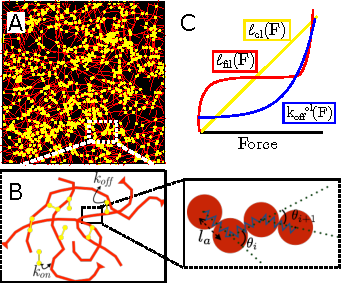
\includegraphics[scale=1.2]{figs/t0.pdf}
  \caption{\label{fig:t0}Computational actomyosin network representation.
  (A) Initial configuration of an assembly of actin filaments (red) which 
  initially have crosslinkers (yellow, one third shown) placed at intersections.
  Cell size is $(75\mu m)^2$. 
  (B) Zoom in of the network revealing that crosslinkers can attach and detach 
  to actin filaments, as well as the bead-spring filament representation of 
  actin described in Methods.
  (C) Schematic of the load dependent detachment rate of crosslinkers, the 
  linear stiffness of crosslinkers, and the nonlinear force extension curve for
  filaments.
  }
\end{figure}
We have quantified the structural rearrangements inherent in bundling by the 
emergent density heterogenity and local alignment. 
Density heterogenity, is measured using the radial
distribution function of actin filaments  $g(r) = P(r)/(2\pi r \delta r\rho)$ 
where $P(r)$ is the probability that two beads on different filaments are 
separated by a distance $r$, $\delta r =0.05 \mu m$ is the bin size and 
$\rho = 500/(75\mu m)^2$ is the number density. \Cref{fig:bundle}B showns that 
for the a bundled configuration the width of the peak of $g(r)$ increases over 
time indicating that more actin filaments are brought closer together. 
Local alignment of actin filaments is measured via the $2D$ nematic order 
parameter $s_2=2\langle\cos^2{\phi_i}\rangle-1$, where $\phi_i$ is the angle 
between a filament link and its local director, defined as the average angle of 
links less than a distance of $1\mu m$.
\par
\Cref{fig:bundle}C shows that $g(r)$ for the final configuration ($t=200s$) 
shows a non-monotonic dependence on crosslinker detachment rate. 
Similarly, \Cref{fig:bundle}D, shows that over time, the nematic order of these
more bundled networks increases to a higher value than the lower bundled
networks. Together, \Cref{fig:bundle}C-D indicate that a low disassociation rate
does not allow for significant restructuring from the 
initially random configuration, and a high disassociation rate will not yield 
long-lived stable structures. However, at intermediate values of $k_{off}^{cl}$,
the filaments self-assemble into a stable, thickly bundled network. This 
relationship is in contrast to the dependence of bundling on crosslinker density, 
which as shown in the Supplement indicates that more crosslinkers yield more 
bundling. 
\par
\begin{figure}[H] 
  \centering
  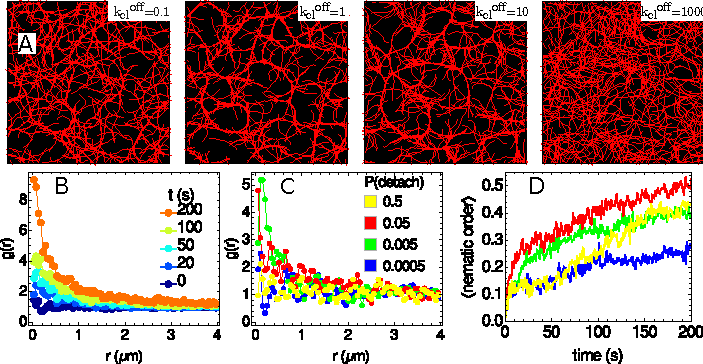
\includegraphics[scale=1.2]{figs/bundling/full_figure.pdf}
  \caption{%
  \label{fig:bundle}%
  Dependence of network bundling on crosslinker detachment rate.
  (\textbf{A}) Network configuration at $t=200s$ for varying disassociation 
  constants of crosslinks (not shown). Filaments are shown in red. 
  (\textbf{B}) Radial distrbiution function of beads on an actin filament for 
  the $k_{off}=20 s^{-1}$ at various times throughout the simulation. 
  (\textbf{C}) Radial distribution function of actin filaments at $t=200s$ for 
  varying $k_{cl}^{off}$.  
  (\textbf{D}) Local ematic order of actin filaments as a function of time for 
  the same values of $k_{cl}^{off}$.  
}
\end{figure}
\subsection{Cooperative sorting of filament polarity by molecular motors}
Molecular motors are modeled as active crosslinkers such that a bound head 
precessively walks toward the barbed end of the filament with load dependent 
speed and kinetic (see Methods for details).
This implementation allows for active filament sliding and filament buckling, 
as elucidated in \Cref{fig:toys}, 
both of which are instrumental for actomyosin contractility \cite{murrell2012}.
In large networks, motors can translocate across filaments, induce filament 
buckling, and also enhance network connectivity\cite{murrell2014}. 
\begin{figure}[H] 
  \centering
  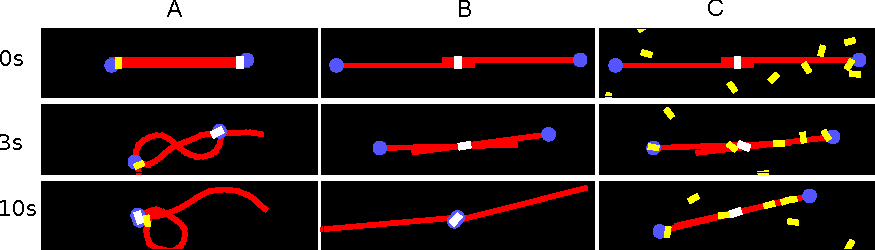
\includegraphics[width=\textwidth]{figs/minimal.pdf}
  \caption{\label{fig:slide}
  \label{fig:toys}%
  Time series of three antiparallel $10\mu m$ filaments (red) interacting with a
  minimal set of motors (white) and crosslinkers (yellow) for $10s$. Barbed ends
  of filaments are marked by a blue dot.  
  (A) Filaments are semiflexible ($21$ bead-spring chain) and pinned on the left
  by a crosslinker, so the motor-filament interaction yields contraction via buckling. 
  (B) Filaments are rigid ($2$-bead-spring chains) and unpinned, so 
  motor-filament interaction yields unimpeded sliding of filaments. As a result,
  they transition from an initially extended state, to a contracted state
  at $t=3s$ and back to a fully extended polarity sorted state at $t=10s$.
  (C) Filaments and motor are the same as (B) but with a population of
crosslinkers near the filaments that arrests the filaments in a contracted state. } 
\end{figure}
To isolate the role of active motors on assemblies of semiflexible filaments,
the actin assembly in \Cref{fig:t0} was generated without crosslinkers at
filament intersections, but with $0.5\mu m$ long motor minifilaments
scattered uniformly throughout the simulation cell. In these simulations, the 
motor duty ratio was kept near unity to replicate the behavior of a myosin 
minifilament, while the density of motors was varied between different
simulations. The results, shown in \Cref{fig:polarity_sorting}, indicate that at
higher motor densities, filaments are sorted by polarity, but are 
not clustered in space. Motors aggregated on the barbed ends of filaments
and thereby brought the different barbed ends together to form asters.
The magnitude of polarity sorting was measured by calculating the contribution 
to the radial distribution function by the barbed ends of actin filaments.
This value, $g(r_{barb}$ is shown in \Cref{fig:polarity_sorting}B and peaks at
significantly higher values than $g(r)$. It is clear from this 
figure that the degree of polarity sorting is highly dependent on motor density.
\par
A secondary peak is visible in \Cref{fig:polarity_sorting} at 
$r_{barb}\approx0.5\mu m$, which the rest length of the the molecular motors. 
This indicates that the motors responsible for polarity sorting remain at the 
center of asters. We calculate the average distance of a bound motor from the 
barbed end of filament to which it was bound to verify that this is the 
mechanism of polarity sorting. 
As seen from \Cref{fig:polarity_sorting}C-D, increasing motor density had the
effect of decreasing this distance, indicating a larger magnitude of polarity
sorting. Thus, motor density tunes the magnitude of polarity sorting in 
assemblies of motors and filaments. Motor-filament affinity also plays an 
important role (see Supplement) where we have shown that the most polarity 
sorted networks emerge from intermediate values of motor detachment. 
\begin{figure}[H] 
\centering
    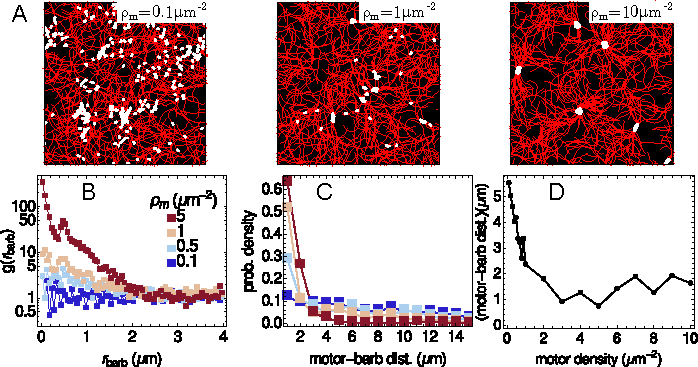
\includegraphics[scale=1.2] {figs/polarity_sorting/ps_fig.pdf}
  \caption{%
  \label{fig:polarity_sorting}%
  (A) Networks at their polarity sorted end configuration ($t=96s$). 
  Filaments are shown in red, motors in white. A maximum of $1000$ motors are
  shown in each case.
 (B) Radial distribution function for barbed ends ($t=96s$) shows a strong 
 dependence on motor density. For $\rho_m=5\mu m^{-2}$, a prominent secondary 
 peak is also visible at the motor rest length $l_m=0.5\mu m$.
 (C) Probability density of the distance of an attached motor
   head from the barbed end of the filament to which it is attached for the same
   simulations.
 (D) The average distance of a motor head from the barbed end as a function of
 motor density.
 } 
 \end{figure}
\subsection{Contractility emerges from competition between bundling and polarity sorting}
\par
When both crosslinkers and motors are mixed with semiflexible filaments, the
assemblies become contractile. To elucidate this behavior, actin filament 
assemblies were initialized (see \Cref{fig:t0}) with crosslinkers at their
intersections with motors scattered uniformly throughout the cell. The motor
density varied between simulations from $0.1-10\mu m^{-2}$. The crosslinkers 
were kept sticky with a low duty ratio, while the motors were highly active with
a high duty ratio. This ensured that connectivity of the network was almost
exclusively controlled by crosslinkers while force generation was controlled by
motors. 
\par
The results of these simulations and the final network configurations can be
seen in \Cref{fig:contract}. The net contractility was measured by
interpolating a velocity field from the displacement vectors of filament beads
from each simulation snapshot, 
measuring the divergence at each point on the vector field, and summing the 
values. A negative total divergence of a given snapshot indicates at that time
the network was contractile. As evident in \Cref{fig:contract}B
higher motor density leads to larger contractility. \Cref{fig:contract}C-D shows
that actin buckling, here measured as the change in the end to end distance
$\Delta s$ of an actin filament:
\begin{equation} 
  \Delta s = \left(1 - {|r_{15}-r_0|\over\sum_{i=1}^{15}{|r_i-r_{i-1}|}}\right) 
  \label{eqn:fil_strain}
\end{equation} 
correlates with contractility, suggesting that the primary mechanism driving
contractility in these flexible networks is filament buckling, as observed 
in experiment \cite{murrell2012}. Networks with low motor densities and extremely
low motor disassocation rates (both with and without crosslinkers) were also 
shown to be contractile, as seen in the supplement.
\begin{figure}[H] 
  \centering
  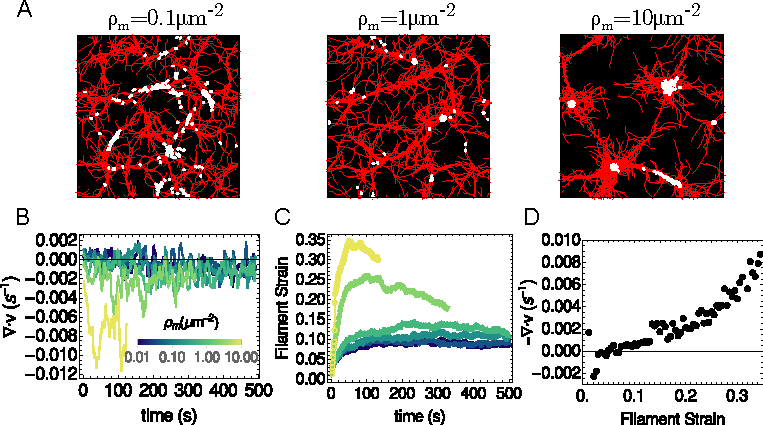
\includegraphics[scale=1.2]{figs/divergence/div_fig.pdf}
  \caption{%
  \label{fig:contract}%
  Assemblies with motors and crosslinkers yield contraction.
  (A) Networks configurations at their largest contractile strains for different
  motor densities. Filaments are shown in red, and motors in white. Only $1000$
  motors are shown in each case.
  (B) Spatially averaged divergence of filament flow field as a function of time
  for networks of varying motor density. 
  (C) Average filament strain (defined in \Cref{eqn:fil_strain}) as a function
  of time for the same networks. 
  (D) Correlation between filament strain and the network strain
  averaged over bins of size $0.005$ for all motor densities
 } 
\end{figure}  
\section{Discussion}
The goal of this paper is to introduce a framework that could accurately and
efficiently simulate active networks of filaments, motors, and crosslinker 
proteins and predict the various structural and mechanical phases of the system.
We have successfully shown that crosslinkers can bundle filaments into thick,
connected networks, motors can sort filaments into structures of homogenous 
polarity, and both can work together to yield actomyosin contraction. We have
characterized the bundled networks via their local alignment, polarity sorted 
networks by the radial distribution function of filament barbed ends, and 
demonstrated contractility by measuring instantaneous network divergence. 
We summarize these results in \Cref{fig:phases}.
\begin{figure}[H]
  \centering
  \includegraphics[scale=0.8]{figs/phase_diagram.pdf}
  \caption{Structural phases of crosslinked actomyosin networks. For blue 
    data points, $\rho$ and $P(detach)$ parameterizes the crosslinkers, 
    while for red and black curves, they parameterize the motors.
  (A) Nematic order of structures emergent from a range of densities and 
  rates for motors and crosslinkers. 
  (B) The probability that filament barbed ends are separated by less
than $1\mu m$ with respect to the probability that arbitrary filament positions 
are separated by less than $1\mu m$.
(C) Total divergence of these networks. Extremely low values at low detachment 
rates indicate that the network was ripped apart.
(D) Phase diagram of all networks at all times. Bundling is measured via nematic
order, polarity sorting as $P(r_{barb})/P(r)$ and contractility as total 
divergence. }
  \label{fig:phases}
\end{figure}
\Cref{fig:phases}A shows that we have characterized bundling using the nematic 
order parameter and that the most locally aligned networks occur when only 
crosslinkers are present. 
This alignment can be tuned by varying both crosslinker density and 
crosslinker detachment rate. For networks with both motors and crosslinkers, 
bundling occurs when motors have a high detachment rate, as the polarity sorting
mechanism is dominated by the bundling mechanism. 
In \Cref{fig:phases}B, we have measured polarity sorting by calculating 
the probability that two filament barbed ends are separated by a 
distance of less than $1\mu m$ with respect to the probability that arbitrary 
positions on a filament are separated by a distance of less than $1\mu m$. 
In this case motors are the key restructuring agent, and higher motor density
yields a stronger polarity sorting effect. The introduction of a small 
population of crosslinkers inhibits this effect slightly, as seen from the black
curve in the left hand plot of \Cref{fig:phases}B, and contraction begins to 
dominate. Network contraction dependence on density and detachment rates 
is measured via the total divergence (summed over space and time) 
shown in \Cref{fig:phases}C, where it is clear that the combination of 
motors and crosslinkers yields the highest values of contraction and that one
can tune this effect by varying motor density and motor detachment rate. 
We used theses order parameters to develop a phase diagram (\Cref{fig:phases}D)
and show that bundling, and polarity sorting, are distinct structural phases
which can couple to yield contractile behavior. 
\par
Each of these structural organization techniques have distinct {\em in vivo}
biomechanical applications. 
Actin bundles can function as force chains to propogate stress large distances
across the cell, and bundled networks can be used to stabilize the cell 
interface, which may be necessary for the formation of an immunological synapse 
\cite{comrie2015}. Polarity sorting can yield directed networks useful for long 
distance transport of 
material across the cell. Actomyosin contraction is necessary for diverse
cell-morphology phenomona including motility and division.
\par
Other actomyosin models have explored the driving mechanisms behind
contractility and structure formation. Dasanyake, et. al., extended the
equilibrium, $2D$ crosslinked rigid filament network model in \cite{head2003} to
include a term in the potential energy that corresponded to myosin motor
activity, and observed the emergence of force chains that transmit stress
throughout the network\cite{dasanyake2011}. Wang and Wolynes \cite{wang2012}
model the F-actin networks as a graph of crosslinkers (nodes) and rigid actin
filaments (edges) in which myosin motor activity is simulated via antisymmetric
kicks along the filaments and predict a binary phase diagram of networks which
are either contractile or not as a function of cross linker and myosin
densities. While the simplicity of these models is intriguing, they do not
account for explicit filament buckling, and their integration is performed via
Monte Carlo, more applicable to structure formation than dynamics.
Nedelec used dynamic simulations of ensembles of filaments
and motor proteins to explore aster formation in microtubule-kinesin assemblies,
as well as motility and contractility in actomyosin
\cite{nedelec2002,nedelec2007,ennomani2016}. 
Kim used an agent based approach of filaments, motors and crosslinkers, to
explore a variety of topics, including bundling via parallel actin crosslinkers 
and force generation by myosin motors\cite{kim2009b, kim2014}. As seen in
Methods, we have benefited from the computational techniques explored in each of
these theoretical models. We have contributed to this area by showing that a 
single model can capture many relevant biophysical structures, precisely 
quantifying these behaviors and showing how to tune them via experimentally 
manipulateable physical parameters. 
\par
While our model is thorough in what it aims to simulate it is limited by a few
experimental observations that are currently not implemented. First, the
structure of myosin minifilaments is significantly more complex than a two
headed spring. As mentioned, these minifilaments have dozens of heads, which
allows them to walk along multiple filaments and could result in subdiffusive
behavior \cite{scholz2016} and significantly increase local network elasticity
\cite{murrellTalk}.
Another limitation of our system is that the actin filaments are static, and
will not polymerize, depolymerize or sever. Within actomyosin assays it is clear
that recycling of actin monomers and to a lesser degree, filament severing 
plays an important role in contraction\cite{murrell2012}. Within the
cytoskeleton, actin treadmilling is also important for shape production.
Additionally, these simulations are all run in $2D$ and without steric
interactions, and dimensionality and volume exclusion may play important roles. 
While we intend to address and investigate these limitations in future works, we
believe that the successful benchmarking of the simulation at various levels is
a significant argument in favor of the current setup.
\par 
There are still many unanswered questions regarding self-organization in
actomyosin networks that we hope can be addressed using this simulation, such as
how actomyosin controls the shape of cell membranes, and how they form force
propogating chains across the cytoskeleton\cite{fraley2005,dasanyake2011}. 
In particular, it is significantly easier to measure internal active forces and
energies in simulation than in experiment, so we expect this model will aid the
process of isolating the particular mechanisms involved in restructuring these
polymer assemblies. We stress, however, that the applicability of such a
simulation package reaches beyond studying the phases of actomyosin networks.  
We believe this simulation can shed light on the mechanics and dynamics of 
a variety of active polymer assemblies.
\par
Similar networks that involve other proteins also exist in the
cytoskeleton, such as microtubule-kinesin-dynein networks and could be
investigated using this simulation methodology. Furthermore, the cytoskeleton
demonstrates how populations of simple machines can self assemble into active
materials with useful mechanical properties, and one can use this simulation to
efficiently design these types of self assembled materials. Thus, the
non-equilibrium molecular dynamics framework of this simulation can be used to
model and study many open questions in active matter and biophysics.
\section{Methods}  
\subsection{Actin Filaments}
Actin filaments are treated as a worm-like chain, with each filament represented as a set of $N+1$ beads connected by $N$ harmonic springs (links), with an additional harmonic angular potential applied on the $N-1$ angles along the chain, as depicted in \Cref{fig:filament}(A). The linear springs 
penalize stretching of individual subunits and the $N-1$ angular harmonic springs penalize bending and enforce the length scale over which the filaments are semi-flexible. 

The internal forces on actin filaments can be obtained from the gradient of the potential energy $U_f$
\begin{eqnarray}
  U_f &=& U_{stretch} + U_{bend}\\
  U_{stretch}&=&{k_a\over2}\sum_{i=1}^{N}{(|d_i| - l_a)^2}\\\nonumber
  U_{bend}&=&{\kappa_B\over 2l_a}\sum_{i=2}^N{\theta_i^2}\\\nonumber
  \label{eqn:Ufil}
\end{eqnarray}
where $d_i = r_i-r_{i-1}$, $\theta_i = \arccos{\left({d_i\cdot d_{i-1}\over |d_i||d_{i-1}|}\right)}$, $k_a$ is the
stretching force constant, $\kappa_B$ is the bending modulus, and $l_a$ is the equilibrium length of a
link. 
\par
For a confined semiflexible filament, it has been show that for a polymer of a given persistence length $L_p$, the shortest length that should be considered as unbending ($l_a$) is given by $l_a\approx A^{2/3}L_p^{1/3}$ where $A$ is a length scale associated with the confinement of the
filament \cite{odijk1983}. In these simulations, filaments were confined by nearby motors and crosslinkers. Since the smallest motor or crosslinker density used was $\rho_m=0.1\mu m^{-2}$, $A\ge1/\sqrt{0.1\mu m^{-2}}\Rightarrow l_a\ge5\mu m$. In general, we used $l_a=1\mu m$.
The bending force constant is derived from the persistence length $L_p$ such that
$\kappa_B = L_p k_B T$ where $k_B$ is Boltzmann's constant and $T$ is the temperature \cite{rubinstein}. Experimentally,
the stretching force constant has been measured to be in the approximate range $k_a=40-70pN/nm$ \cite{kojima1994, higuchi1995}; however, simulating a
network of filaments with this large of a stiffness is computationally inefficient since the maximum timestep of a
simulation is inversely proportional to the largest stiffness in the simulation. Therefore, we chose ${\kappa_B\over
l_a} <<k_a$, so that the filaments were still much easier to bend than to stretch, enabling us to run simulations of
experimentally relevant dimension. We show that our simple filament model exhibits expected behavior for a semiflexible
filament in the next section and we have further verified that $k_a$ did not effect the persistence length of the
filament, as seen in the Supplement. 
\par
Since actin bending is instrumental for actomyosin contraction, and simulating precise bending moduli is non-trivial, we tested our filaments by measuring spatial and temporal fluctuations and comparing with theoretical predictions.
In a two dimensional WLC, a bending of two adjacent segments is expected to result in a local change in free energy of ${\kappa_B\over2l_a\theta_i^2}$, and it is predicted that \cite{frontali1979}
\begin{equation}
  \langle\theta^2(l)\rangle = {l\over L_p}
  \label{eqn:thsq}
\end{equation}
\begin{equation} 
  \langle\cos(\theta(l))\rangle = \exp{(-l/2L_p)}
  \label{eqn:costh}
\end{equation} 
where $\theta(l) = \theta_j - \theta_i$ where $1<i<j\le N$, $l = l_a(j-i)$ and $L_p$ is the persistence length. To test our model against these equations, we simulate $100$ filaments of $L=200\mu m$ and $\kappa_B=0.08 pN\mu m^2$ at $T=300K$ for $T_f = 100s$ and measured the resulting filament configuration every $1s$. We discard the first $10$ seconds of each simulation to allow equilibration, and we used only the middle $150 \mu m$ of the filament to calculate these correlation functions.
%For each of the $90000$ filament configurations, and for each $l\in{0,1,2,..,150}\mu m$,
%$\theta^2(l)$ and $\cos(\theta(l))$ were calculated, and their respective averages are plotted in 
%\Cref{fig:avgTh}, along with the expected behavior given the input $\kappa_B$.  
We have also shown (Supplement) that the measured persistence length, obtained by performing a least squares fit to
plots of $\log{(\langle cos(\theta(l))\rangle )} $ for various values of $\kappa_B$ yields the expected result over at
least $3$ orders of magnitude. Further measurements of the persistence length as well as verifications of its
independence on other filament parameters is available in the supplement.
\par
An additional prediction for semiflexible filaments is the scaling of fluctuations with time. 
Fluctuations transverse to the filament orientation have been 
shown to increase as a function of time as $\langle dr_{\perp}^2\rangle\propto t^{3/4}$ while longitudinal fluctuations have been shown to follow the power law
$\langle dr_{||}^2\rangle\propto t^{7/8}$ \cite{everaers1999}. To tests these predictions, we followed the procedure outlined in
\cite{everaers1999} and generated $N = 100$ initial filament configurations of a $20\mu m$ filament. For each configuration we ran $M = 100$ simulations of the filament fluctuating for $1s$. At each time step we collected the $2N$ positions of the filament ends, $r_e(t)$. We then calculated the eigenvalues of the covariance matrix $cov(r_e(t)\cdot \hat{i},r_e(t)\cdot \hat{j})$ where
$i,j\in\{x,y\}$.
The larger eigenvalue $\lambda_1(t)$ corresponds to the slower longitudinal fluctuations
(i.e., $\lambda_1(t)\propto t^{7/8}$) while the smaller eigenvalue corresponded to the faster perpendicular fluctuations
($\lambda_2(t)\propto t^{3/4}$). We show  in \Cref{fig:filament}(C) that the our simulation exhibits scaling of these eigenvalues in good agreement with the prediction of Ref. \cite{everaers1999}.
\begin{figure}[H] 
  \centering
   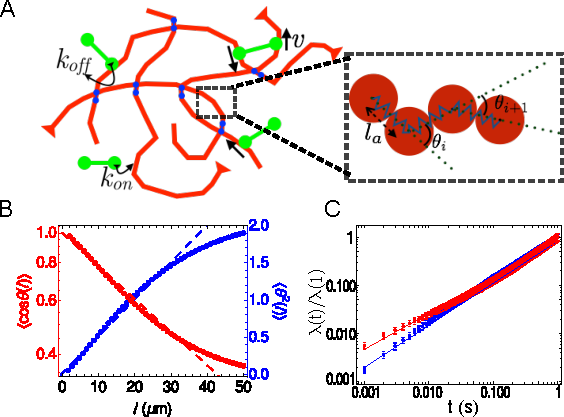
\includegraphics[scale=1]{figs/filament/pl_fig.pdf}
  \caption{\label{fig:filament}
  Correlations of actin filaments in space and time.
  (A) Decorrelation of tangent vectors (red dots) and fluctuations in angles between links (blue dots) 
  as a function of the arc length between them. Red dashed
  line is $e^{-s/2L_p}$ shows the expected behavior from the input bending modulus of $0.08 pN-\mu m^2$ and blue
  dashed line has slope $1/L_p$.
  (B) Eigenvalues of covariance matrices for the positions of endpoints of filaments as a function of time. We analyze fluctuations of $N=100$ filaments, with each point the average over the $2N$ eigenvalues for $\lambda_1(t)$ and $\lambda_2(t)$ and error bars showing the standard deviations for the
distribution of these values. Blue
  dots shows the longitudinal fluctuations and the red dots shows the transverse fluctuations. Red dashed line is
  $t^{3/4}$ and blue dashed line is $t^{7/8}$ as predicted by \cite{everaers1999}. 
}
\end{figure} 
\subsection{Crosslinkers}
Crosslinker proteins dynamically connect actin filaments, thereby propogating force from one to
another. Thus model crosslinkers, must be able to attach and detach from actin filaments,
and be compliant in order to propagate force. They are therefore modeled as hookean springs, with stiffness
$k_{cl}$ and rest length $l_{cl}$. Like actin filaments, the Young's modulus of
most crosslinkers is significantly higher than would be reasonable to simulate; therefore we set $k_{cl} = 1-100pN/\mu m$ was
so that the bending mode of actin filaments was signicantly softer than the stretching mode of
crosslinkers. Their rest length $l_{cl}$ differs by the type of cross-linker and ranges from $~10 nm$ for fascin to $150 nm$
for filamin. 
\par
At each time step of the simulation an unattached crosslinker head is allowed to attach to nearby
filaments and an attached crosslinker head can detach. 
The probability of a head attaching to an actin filament is a Gaussian distributed random variable, such that
\begin{equation}
  P_{cl}^{on} = k_{cl}^{on}dt\exp(-r^2/R^2)
  \label{eqn:cl_on}
\end{equation} 
where $r$ is the shortest distance from the head to the actin filament and $R = \sqrt{2k_B T\over k_{cl}}$ 
where $k_B$ is Boltzmann's constant and $T$ is the temperature. 
For crosslinker detachment we assume that the behavior is that of a slip bond, such that a higher
tensile force along the crosslinker backbone will result in a higher probability of detachment. Thus, 
\begin{equation}
  P_{cl}^{off} = k_{cl}^{off} dt\exp{\left(  F x_{cl}/k_B T\right)}  
  \label{eqn:cl_off}
\end{equation}
where $F$ is the force along the crosslinker backbone, and $x_{cl}$ is a characteristic bond length \cite{stam2015}. 
\par
When a crosslinker is bound to a filaments at both ends, it will necessarily be stretched or compressed. 
If it were allowed to relax independently of the actin filaments to which it is bound. 
it would no longer lie on those filaments. Therefore, the tensile force stored on a stretched or compressed
crosslinker is propagated onto those actin filaments via the lever rule outlined in 
\cite{nedelec2002, gordon2012}. Thus, if the tensile force of a motor at point $r_j$ between filament beads $i$ and $i+1$ is
$F_{cl}$, then, 
\begin{eqnarray} 
  F_i &=& F_{cl}\left|\left( {r_j - r_i \over r_{i+1} - r_i }\right)\right|\\\nonumber
  F_{i+1} &=& F-F_i 
  \label{eqn:lever}
\end{eqnarray}
will be the forces on beads $i$ and $i+1$ respectively due to the crosslinker.
\subsection{Motors}\label{sec:methods_motors}
Within the cytoskeleton, tens of myosin II motors aggregate into bipolar ensembles called myosin minifilaments
\cite{stam2015}. While the mechanochemical process through which individual myosin motors walk along actin filaments is complex, 
motility assay experiments have shown that on average bound myosin II heads walk at an unloaded speed of $v_0\approx1\mu m/s$ along actin
filaments\cite{finer1994}. To a first approximation, minifilaments therefore should also 
have a mean speed of $1\mu m/s$ (although see \cite{stam2015} and \cite{walcott2012} for higher order measurements). 
Since myosin also functions to increase the local elasticity of networks wherever it is bound, the myosin is modeled
similarly to a crosslinker, in that it behaves like a hookean spring with two heads, a stiffness $k_{m}$ and a rest
length $l_m$. It should be noted, however, that the two heads of this spring do not correspond directly to individual
molecular myosin heads; rather each of them represents tens of myosin molecules, and their rate constants will reflect
that notion. 
It would be undesirable for a myosin minifilament to stretch, 
since experimentally they have a very high
Young's modulus and it is unlikely that their length would change noticably in the cytoskeleton. Thus we set $k_m\gg\kappa_B/l_a$
so that the bending of actin is still the softest mode. 
The rest length was set to the average length of minifilaments \cite{niederman1975}.
Attachment and detachment kinetics for motors are the same as for crosslinkers, subscripted with $m$
instead of $cl$ in \Cref{eqn:cl_on,eqn:cl_off}. One extra parameter is needed $k_m^{end}$ for the
detachment of myosin from the barbed end of a filament, as detachment from the end is significantly more probable than
from the rest of the filament.
Similarly, force propogation onto minifilaments is done using the lever rule described in \Cref{eqn:lever}.
\par
Unlike crosslinkers, motors process towards the barbed end of actin filaments to which they are bound 
at speeds that vary depending on the tensile force along the crosslinker. 
The relationship between motor velocity and tensile force is modeled linearly, such that the motor head 
will speed up if the minifilament is
compressed (pre-powerstroke) and slow down if the minifilament is stretched (post powerstroke) going to
$0$ when the force on the minifilament is the stall force $F_s\approx 3.85pN$ \cite{nedelec2002, gordon2012}; i.e.,  
\begin{equation} 
  v(F_{||}) = v_0\left( 1-{F_{||}\over F_s}) \right)
    \label{eqn:myo_vel}
\end{equation} 
where $F_{||}$ is the force on the motor, projected along the tangent vector of the
actin filaments.
The minor differences between crosslinkers and motors allow us treat them equivalently, by 
setting $v_0 = 0$ for the crosslinkers.  

\subsection{Dynamics}
We Langevin dynamics to solve for the motion of actin filaments, myosin minifilaments and crosslinkers.
The Langevin equations of motion for a spherical bead of
mass $m$ and radius $R$ at position $r(t)$ at time $t$ can be written,
\begin{equation}
  m\ddot{r}(t) = F(t) + B(t) - 4\pi R\nu \dot{r}(t)
  \label{eqn:lang}
\end{equation} 
where $F(t)$ is the force on the particle due to its interactions and $B(t)$ is Brownian forcing term, to simulate a temperature, $\nu$ is the dynamic viscosity of the bead's
environment, and we have used the Einstein relation for the damping term.  
Since the fastest motion in this simulation is that of the myosin, and a $0.4\mu m$ myosin minifilament moving at
a speed of $1\mu m/s$ in a liquid at least as viscous as water ($\nu_D=10^6\mu m^2/s$ dynamic viscosity) has a very low Reynold's
number ($Re \approx 4*10^{-7}$) we can treat the dynamics in the overdamped limit where the equation of motion is \Cref{eqn:lang} without the acceleration term, i.e. with $m=0$.
Furthermore, in the limit of small $\Delta t$, we may write $\dot{r(t)} \approx {r(t+\Delta t)-r(t)\over \Delta t}$. These two
approximations allow us to rewrite \Cref{eqn:lang} as 
\begin{equation}  
  r(t+\Delta t) = r(t) + F(t)\mu \Delta t + B(t) \mu \Delta t
\label{eqn:overdamped}
\end{equation}
where $\mu = (4\pi R\nu)^{-1}$. For the Brownian term, we use the form of Leimkuhler and Matthews \cite{leimkuhler2012,leimkuhler2013} that has
been shown to minimize deviations from canonical averages in harmonic systems,
\begin{equation}
  B(t)=\sqrt{2k_BT\over\mu \Delta t}\left({W(t)+W(t-\Delta t)\over2}\right)
  \label{eqn:baoab_brownian}
\end{equation} 
where $W(t)$ is a Wiener process, in this case a random number drawn from the normal distribution with mean zero and standard deviation of unity.

\subsection{Environment}
\par
Because the probability of motor attachment decays as a Gaussian function of distance from the filament, it would be highly inefficient to attempt motor attachments with every filament in the simulation.  Rather, we choose to test for connections only within a cutoff distance
$r_c>3R/2$ (where $R$ is defined above as in \Cref{eqn:cl_on}). A grid of lattice size $2r_c$ is drawn in the $2D$ plane of the simulation, and the position of a filament is approximated as the points on the grid nearest to the beads of the filament. Thus, to determine if a motor will bind to a filament at time $t$, it is sufficient to only attempt attachment to filaments that are indexed at the four nearest grid points to a motor. 
\par
In general, we use periodic boundary conditions so as to limit effects of a boundary and to mimic a system larger than the one we simulate. Lees-Edwards boundaries \cite{allen} were used for shearing simulations, and hard wall boundaries have also been implemented.
The value for $\Delta t$ in \Cref{eqn:overdamped} generally depends on both the unloaded myosin speed
$v_0$ and the largest stiffness in the simulation $k_f$. For $k_f = 10pN/\mu m$ and $v_0=1\mu m/s$ a value of $\Delta t = 0.00001 s$ was sufficiently low to solve \Cref{eqn:overdamped} for hundreds of seconds without spuriously generating configurations of very large energy.
The length and width of the simulations were chosen so as to be high enough to avoid boundary artifacts. 
A complete list of simulation parameters used throughout this article is provided in \Cref{tab:params}. 
\begin{table}
  \caption{Parameter Values}
  \centering
  \begin{tabular}{|C{1cm}|L{6cm}|C{2cm}|C{2cm}|C{2cm}|C{2cm}|}
    \hline\hline
    Symbol & Description (units) [ref] & $L_p$ & Shear & Motility Assay & Networks\\
    \hline
    &\bf{Actin Filaments}& & & &\\
    \hline
    $N_B$ & Number of beads & $21-201$ & $16$ & $16$ &$16$\\
    $l_a$ & Link Rest Length ($\mu m$)\cite{odijk1983}& $1$ & $1$ &$1$& $1$\\
    $k_a$ & Stretching Force Constant ($pN/\mu m$) & $0.01-10$ & $10$ & $1$ & $1$\\
    $\kappa_B$ & Bending Modulus ($pN\mu m^2$)\cite{ott1993} & $0.002-5 $ & $0.08$ & $0.08$ & $0.08$\\
    \hline
    &\bf{Myosin Minifilaments}& & \\
    \hline
    $l_m$ & Rest Length ($\mu m$)\cite{niederman1975} & n/a & n/a & 0.5 & 0.5\\
    $k_m$ & Stiffness ($pN/\mu m$)& n/a & n/a & $1$ & $1$\\
    $k^{on}_m$ & Attachment rate at distance $r=0$ ($s^{-1}$)& n/a & n/a &$2-4000$ &$3600$\\
    $k^{off}_m$ & Unloaded head detachment rate ($s^{-1}$)& n/a & n/a & $200$ &$200$\\
    $k^{end}_m$ & Unloaded head detachment rate at the barbed end of the filament ($s^{-1}$)& n/a & n/a &$2000$ &$2000$\\
    $x_m$ & characteristic bond length ($\mu m$) \cite{stam2015}& n/a & n/a & $0.0004$& $0.0004$\\
    $v_0$ & Unloaded speed ($\mu m/s$) \cite{kron1986}&  n/a & n/a & $1$ & $1$\\
    $F_s$ & Stall force of myosin ($pN$)\cite{veigel2003}& n/a & n/a & $3.85$ & $3.85$\\
    \hline
    &\bf{Crosslinkers} & & \\
    \hline
    $l_{cl}$& Rest Length (Filamin) ($\mu m$)\cite{ferrer2008} & n/a &$0.150$ &n/a&$0.150$ \\
    $k_{cl}$ & Stiffness ($pN/\mu m$)& n/a & $1,10$ & n/a& $1$\\
    $k^{on}_{cl}$ & Attachment rate at distance $r=0$ ($s^{-1}$)& n/a & $10^6,10^5$ &n/a &$3600$\\
    $k^{off}_{cl}$ & Unloaded head detachment rate ($s^{-1}$)& n/a & 0 & n/a&$0.2$\\
    $x_{cl}$& characteristic bond length ($\mu m$) & n/a & $0.0004$ & $0.0004$ & $0.0004$ \\
    \hline
    &\bf{Environment} & & \\
    \hline
    $dt$ & Dynamics timestep (s) & $10^{-4}$ & $10^{-6},10^{-5}$ &$2.5\times10^{-4}$ &$2.5\times10^{-4}$ \\
    $T_F$& total simulated time (s) & $100$ & $0.5$ & $100$ & $500$ \\
    $X$, $Y$ & Length and width of assay ($\mu m$)& n/a & $75$ & $50$ & $75$\\
    $r_c$ & Mesh (actomyosin binding site) size ($\mu m$) & $n/a$ & $0.2 $ & $0.2 $& $0.2 $ \\ 
    $T$ & $k_B$ * Temperature ($pN\mu m$)& $0.004$ & $0.004$& $0.004$& $0.004$\\
    $\nu$ & Dynamic viscosity ($mg/(\mu m s)$) & $0.001$& $0.001$& $0.001$& $0.001$\\
    $\gamma$ & Strain (\%) \cite{stricker2010}& n/a& $0.001$&n/a&n/a\\
    $t_{relax}$ & Amount of time between sequential strains (s)& n/a& $0.001$ &n/a&n/a\\
    \hline
  \end{tabular}
  \label{tab:params}
\end{table}



\section{Acknowledgements}  
We thank M. Gardel, J. Weare, C. Matthews, F. Nedelec, F. Mackintosh, and M. Murrell for helpful conversations. This research was supported in part by the University of Chicago Materials Research Science and Engineering Center (NSF Grant No. 1420709). S.L.F. was supported by the Department of Defense (DoD) through the National Defense Science \& Engineering Graduate Fellowship (NDSEG) Program. G.M.H. was supported by an NIH Ruth L. Kirschstein NRSA award (1F32GM113415-01).
\bibliography{actosim}
\bibliographystyle{unsrt}

\beginsupplement
\end{document}
